\section{Errors and Sensitivity}
We summarize the anticipated errors in the determination of the $\pi^0$ polarizability. We assume 
20 days of running on a 5\% radiation length $^{208}$Pb target, 10$^7$ photons/s, and nominal acceptance for $\pi^0 \pi^0$.
Table \ref{errors} summarizes the estimated statistical and systematic errors. In the following we describe each of
these contributions in detail: 

%\end{landscape}
% \begin{landscape}
\begin{table}[bt]
\caption{Uncertainties in the extraction of $\pi^0$ polarizabilities $\alpha_{\pi^0}-\beta_{\pi^0}$.
\label{errors}
}
\begin{center}
\begin{tabular}{|l|l|c|c|}
\hline
\hline
  &  Source  & Uncertainty   \\  \hline \hline
  1 & Statistical uncertainty  &  2.3 \%    \\ \hline
  2 & Flux normalization &  1.5 \%     \\ \hline
  3 & Signal extraction  & 3.0 \%  \\ \hline
  4 & Detector acceptance and efficiency &  3.5 \%   \\ \hline
  5 & Total systematic error  &  4.8\% \\ \hline
  6 & Total error on cross section  &  5.3\% \\ \hline
  7 & Projected error in $\alpha - \beta$ &  41\%  \\ 
 \hline
 \hline
\end{tabular}
\end{center}
\end{table}
%\end{landscape}

\begin{enumerate}

\item
Statistical uncertainty in extraction of the Primakoff signal as determined by the fit shown in the top left plot in Fig.\,\ref{fig:decomposition_PrimNCICeta} (Section\,\ref{sec:signalfit}).

\item
Flux normalization. We have several methods for determining the flux (Section\,\ref{sec:flux}). The Primex-D experiment expects an uncertainty of 1.5\% and we use that as our estimate here.

\item
Systematic uncertainty in extraction of the signal. This contribution is estimated to be 3\% based on differences obtained in the Primakoff signal by varying the amount of background contributions (Section\,\ref{sec:signalfit}).

\item
Detector acceptance and efficiency. We can measure the detector acceptance times efficiency for the process $\gamma \mathrm{Pb} \rightarrow \pi^0 \mathrm{Pb}$ with an accuracy of 3.5\% (Section\,\ref{sec:pi0norm}), which
should allow us to reduce the systematic uncertainty in the acceptance calculation for the process of interest to this level.

\item
Total systematic error (items 2-4): combining the systematic errors in quadrature gives 4.8\%.

\item 
Error on cross section (quadrature sum of items 1 and 5): 5.3\%.

\item
The current estimate by Dai and Pennington (Table II in Ref.\,\cite{Dai:2016ytz}) indicates
that a 13\% determination of
$\sigma(\gamma\gamma\rightarrow\pi^0\pi^0)$ will determine the
combination $\alpha_{\pi^0}-\beta_{\pi^0}$ to a precision of 100\%, i.e., $\Delta(\alpha_{\pi^0}-\beta_{\pi^0}) \sim 7.7\Delta(\sigma$) .
From here we estimate that our uncertainty on $\Delta(\alpha_{\pi^0}-\beta_{\pi^0}) \sim$ 41\%. We note that the basis for extracting the polarizabilities may be improved
in the near future and theoretical effort is being directed specifically toward this goal.

\end{enumerate}

\begin{table}[hbt]
\caption{Approved beam request and running conditions for CPP. NPP would run concurrently.
\label{request}
}
\begin{center}
\begin{tabular}{|l|c|c|c|c|c|c|c|c|}
\hline
\hline
  Running condition  &            \\ \hline
  Days for production running  &   20   \\ \hline
  Days for calibrations &  5       \\ \hline
  Target   & $^{208}$Pb   \\ \hline
  Photon intensity in coherent peak &   10$^7$ photons/s     \\ \hline
  Edge of coherent peak  &  6 GeV   \\ \hline
 \hline
 \hline
\end{tabular}
\end{center}
\end{table}
 
\section{Summary and beam request}
We have investigated the possibility of determining the neutral pion
polarizabilities $\alpha_{\pi^0}-\beta_{\pi^0}$, a quantity for which there are no existing measurements.
Our proposal is to extract the polarizability from a 
measurement of the cross section of the Primakoff reaction $\gamma
\rm{Pb}\rightarrow \pi^0 \pi^0 \rm{Pb}$. We propose to make this
measurement using data taken simultaneously with the CPP\cite{CPPexp}
experiment in Hall D. Table \ref{request} summarizes the approved beam request for the CPP experiment.
The existing GlueX detector has sufficient
resolution and high acceptance for this process. We expect to collect approximately 1800 signal events during the
approved 20 PAC days. The anticipated   uncertainties on
the signal represent a significant improvement over existing data as shown in Fig.\,\ref{fig:sigma_2pi0_figs_4}.
Using the estimate by Dai and Pennington \cite{Dai:2016ytz} we expect to be able to make the first extraction of the 
$\alpha_{\pi^0}-\beta_{\pi^0}$ polarizability with an uncertainty of 41\%.

\begin{figure}[tpb]
\centering
\includegraphics[page=4,width=4.75in]{figures/sigma_2pi0_figs.pdf}
\caption{Estimated uncertainties (systematic and statistical errors are added in quadrature) in determining $\sigma(\gamma\gamma\rightarrow\pi^0\pi^0$) during 20 PAC days running simultaneously with the approved CPP experiment. The data points from the single previous Cristal Ball measurement \cite{Marsiske:1990hx} are shown for comparison.
\label{fig:sigma_2pi0_figs_4}}
\end{figure}





